\documentclass[14pt,a4paper]{extarticle}
\usepackage[T2A]{fontenc}
\usepackage[utf8]{inputenc}
\usepackage[russian]{babel}
\usepackage{geometry}
\usepackage{graphicx}
\usepackage{float}
\usepackage{listings}
\usepackage{xcolor}
\lstset{basicstyle=\ttfamily\small,breaklines=true,frame=single,columns=fullflexible,backgroundcolor=\color{black!3}}
\geometry{left=30mm,right=15mm,top=20mm,bottom=20mm}
\setlength{\parindent}{1.25cm}
\sloppy
\begin{document}
\begin{titlepage}\begin{center}
САНКТ-ПЕТЕРБУРГСКИЙ НАЦИОНАЛЬНЫЙ\\ ИССЛЕДОВАТЕЛЬСКИЙ УНИВЕРСИТЕТ ИТМО
\vspace{1.5cm}

Дисциплина: Бэк-энд разработка
\vspace{1.5cm}

\textbf{Отчет}
\vspace{0.5cm}

Лабораторная работа 6
\vspace{0.5cm}

\textbf{Настройка системы мониторинга ресурсов}
\vfill
\begin{flushright}Выполнил:\\ Цатинян Артём\\ Группа БР1.2
\vspace{0.8cm}

Проверил:\\ Добряков Д. И.\end{flushright}
\vfill Санкт-Петербург\\ 2026 г.
\end{center}\end{titlepage}
\section{Задача}
Настроить мониторинг виртуальной машины и микросервисного приложения с помощью Grafana. Дашборд должен показывать загрузку процессора, памяти, диска и сети, доступность сервисов и журналы контейнеров.
\section{Ход работы}
\subsection{Состав системы}
Для системы бронирования ресторанов подготовлен отдельный проект Docker Compose. Node Exporter предоставляет метрики виртуальной машины. Prometheus собирает их и результаты HTTP-проверок Blackbox Exporter. Grafana Alloy обнаруживает контейнеры через Docker API и отправляет журналы в Loki. Grafana объединяет метрики и журналы на дашборде.

Система запущена на виртуальной машине Ubuntu 24.04 из ЛР5. Контейнеры мониторинга и приложения соединены через существующую сеть Docker restaurant-booking\_default. Grafana доступна на порту 3030 виртуальной машины. Для хранения метрик, журналов и настроек используются отдельные Docker volumes.

Контролируются четыре сервиса: identity, catalog, booking и review. HTTP-проверка обращается к OpenAPI каждого сервиса и ожидает успешный ответ. Эта проверка показывает доступность HTTP-интерфейса, но не подтверждает корректность всех бизнес-сценариев.
\subsection{Конфигурация}
В состав работы входят compose-файл, конфигурация Prometheus, модуль HTTP-проверок, конфигурация сбора журналов и файлы автоматической настройки источников данных и дашборда Grafana. Метрики собираются с интервалом 15 секунд, срок хранения Prometheus составляет три дня. В дашборде предусмотрены панели процессора, памяти, файловой системы, дискового и сетевого ввода-вывода, доступности сервисов и журналов контейнеров.

В Prometheus настроены задания сбора собственных метрик, метрик узла и доступности сервисов. Для проверки HTTP используется blackbox-exporter: адрес сервиса передаётся через параметр target, а результат сохраняется в метрике probe\_success. Проверка выполняется по пути /v3/api-docs каждого сервиса.

Node Exporter запущен с сетевым пространством виртуальной машины, а её корневая файловая система подключена для чтения. Это позволяет собирать метрики самой ВМ. Для журналов Alloy получает список контейнеров через Docker API и присваивает записям метку container; Loki принимает записи, Grafana отображает их по запросу \texttt{\{job="docker"\}}. Доступ к Docker API предполагает значительные права на узле, поэтому конфигурация рассчитана на учебную локальную среду.

Источники данных Prometheus и Loki, а также дашборд создаются автоматически при запуске Grafana из файлов provisioning. Дашборд включает семь панелей: процессор, память, файловая система, сеть, дисковый ввод-вывод, доступность сервисов и логи.
\subsection{Проверка}
После переноса файлов на виртуальную машину выполнен запуск \texttt{sudo docker compose up -d}. Команда \texttt{docker compose ps} показала шесть работающих компонентов системы мониторинга.
\begin{figure}[H]\centering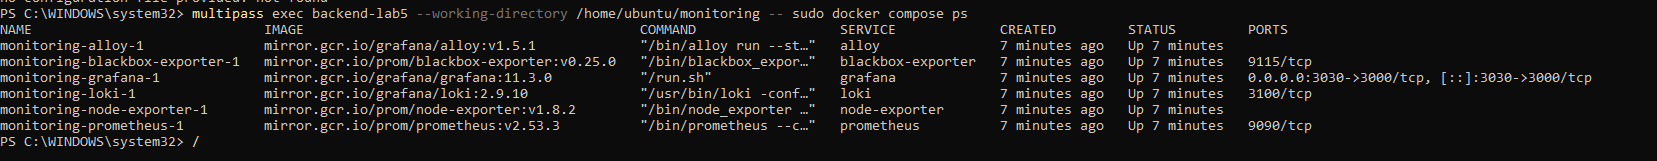
\includegraphics[width=\textwidth]{screenshots/containers.png}\caption{Состояние контейнеров мониторинга}\end{figure}

В интерфейсе Grafana настроенные источники данных отображаются в списке, тестирование соединения с каждым завершилось успешно.
\begin{figure}[H]\centering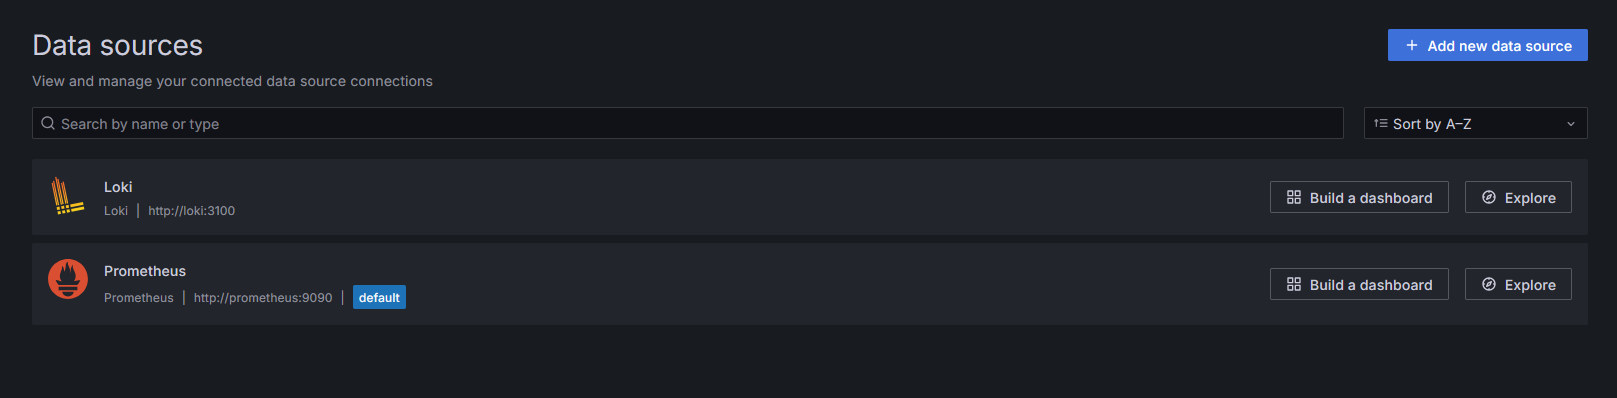
\includegraphics[width=\textwidth]{screenshots/datasources.png}\caption{Источники данных Grafana}\end{figure}
\begin{figure}[H]\centering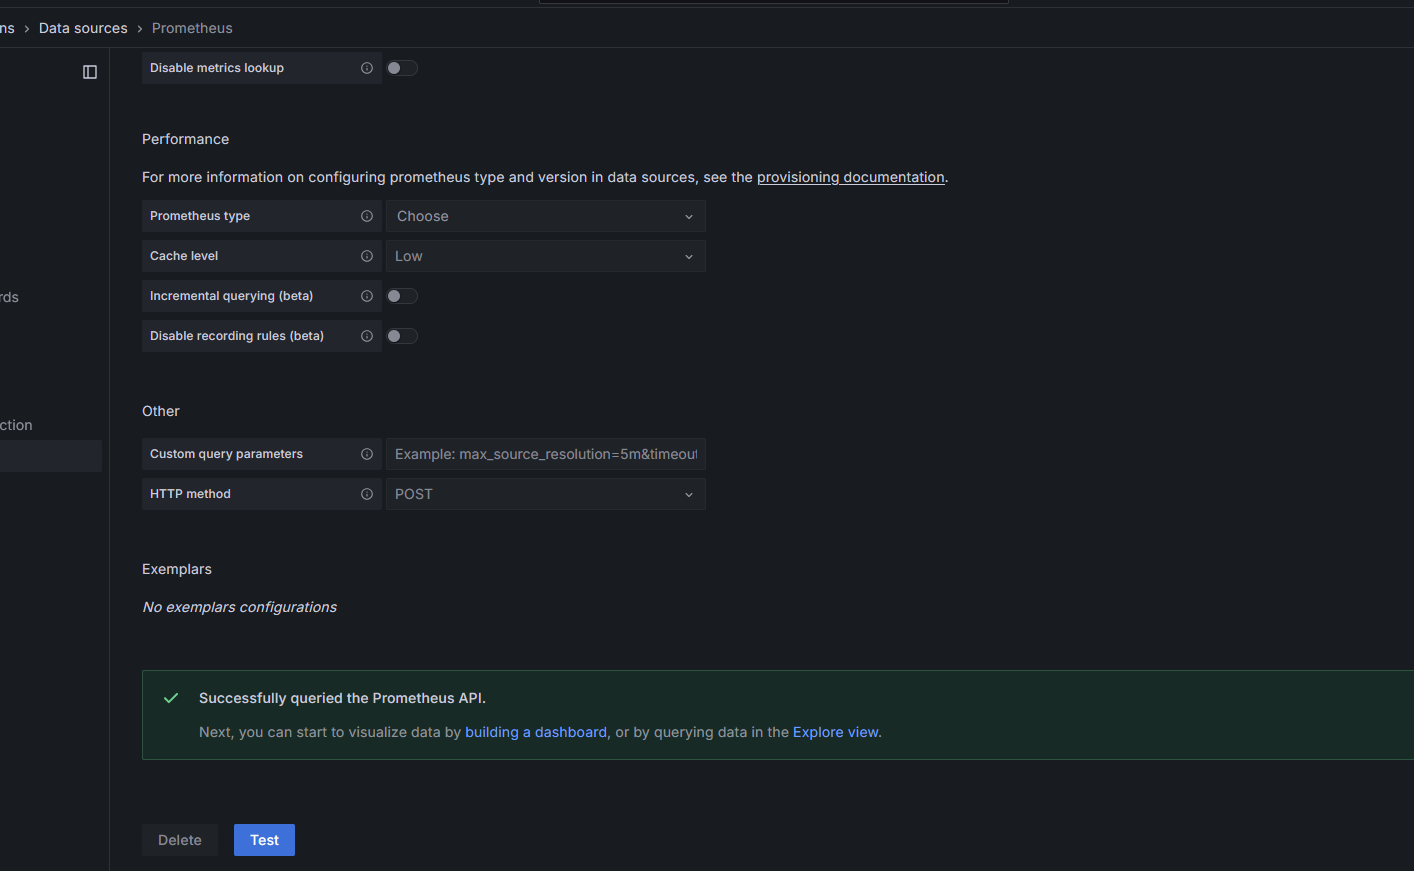
\includegraphics[width=\textwidth]{screenshots/prometheus.png}\caption{Проверка подключения к Prometheus}\end{figure}
\begin{figure}[H]\centering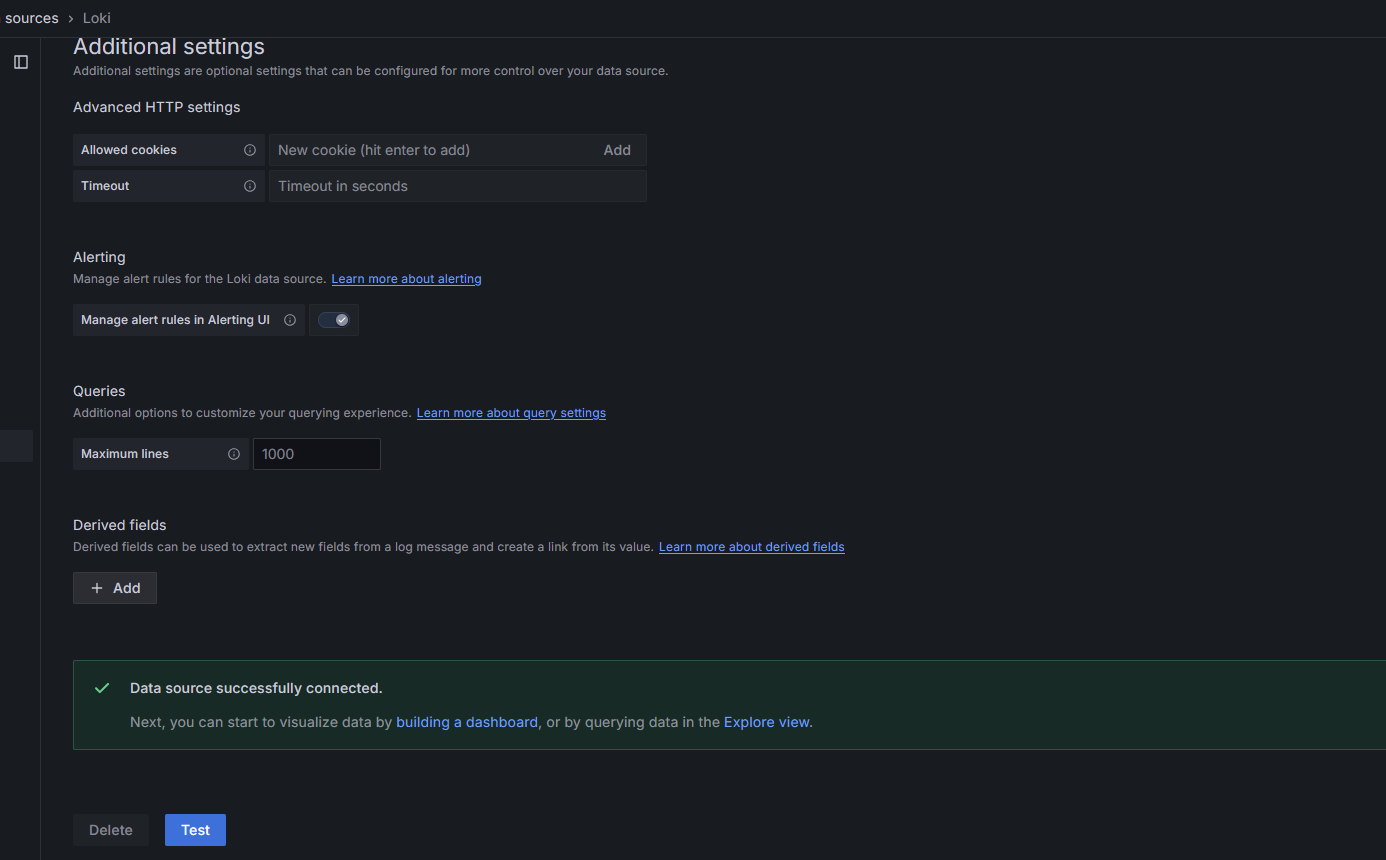
\includegraphics[width=\textwidth]{screenshots/loki.png}\caption{Проверка подключения к Loki}\end{figure}

Дашборд отображает собранные показатели загрузки процессора и памяти, заполнения файловой системы, сетевого и дискового ввода-вывода. Все четыре проверки сервисов на момент снимка показывают состояние «Доступен». На панели журналов отображаются записи контейнеров; на представленном снимке видны, в частности, журналы компонентов мониторинга.
\begin{figure}[H]\centering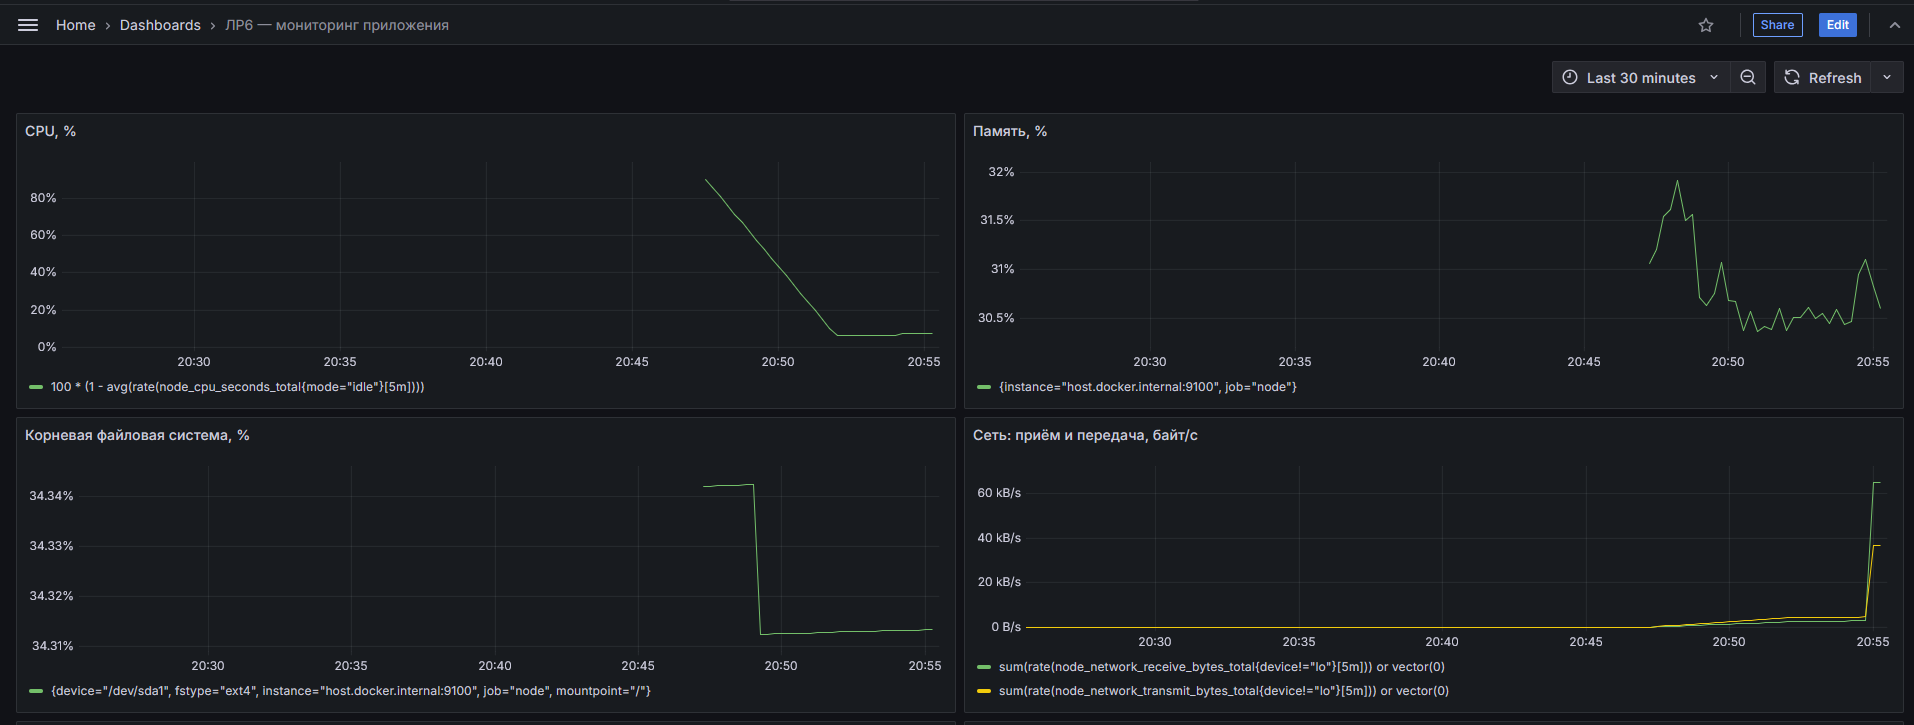
\includegraphics[width=\textwidth]{screenshots/metrics.png}\caption{Метрики ресурсов виртуальной машины}\end{figure}
\begin{figure}[H]\centering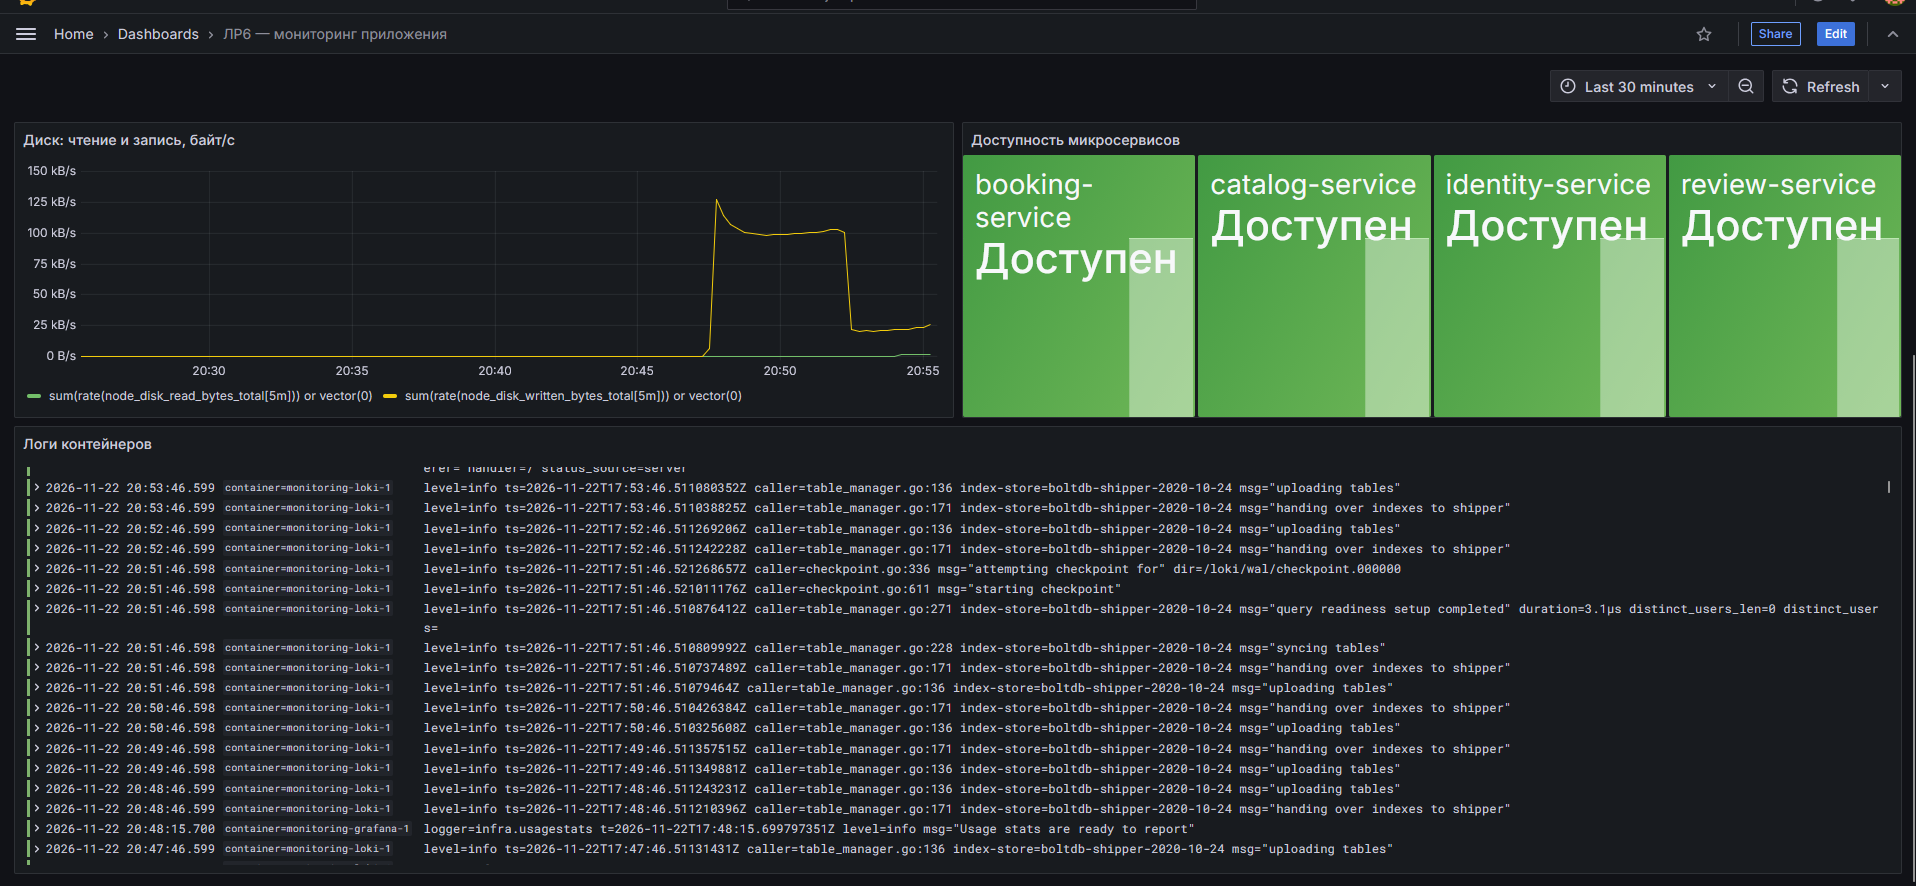
\includegraphics[width=\textwidth]{screenshots/status-logs.png}\caption{Доступность микросервисов и журналы контейнеров}\end{figure}

В Grafana Explore дополнительно выполнен запрос к Loki с фильтром по контейнеру identity-service. В результате получены записи запуска приложения, работы Liquibase и обработки запросов, что подтверждает поступление журналов этого сервиса в Loki.
\begin{figure}[H]\centering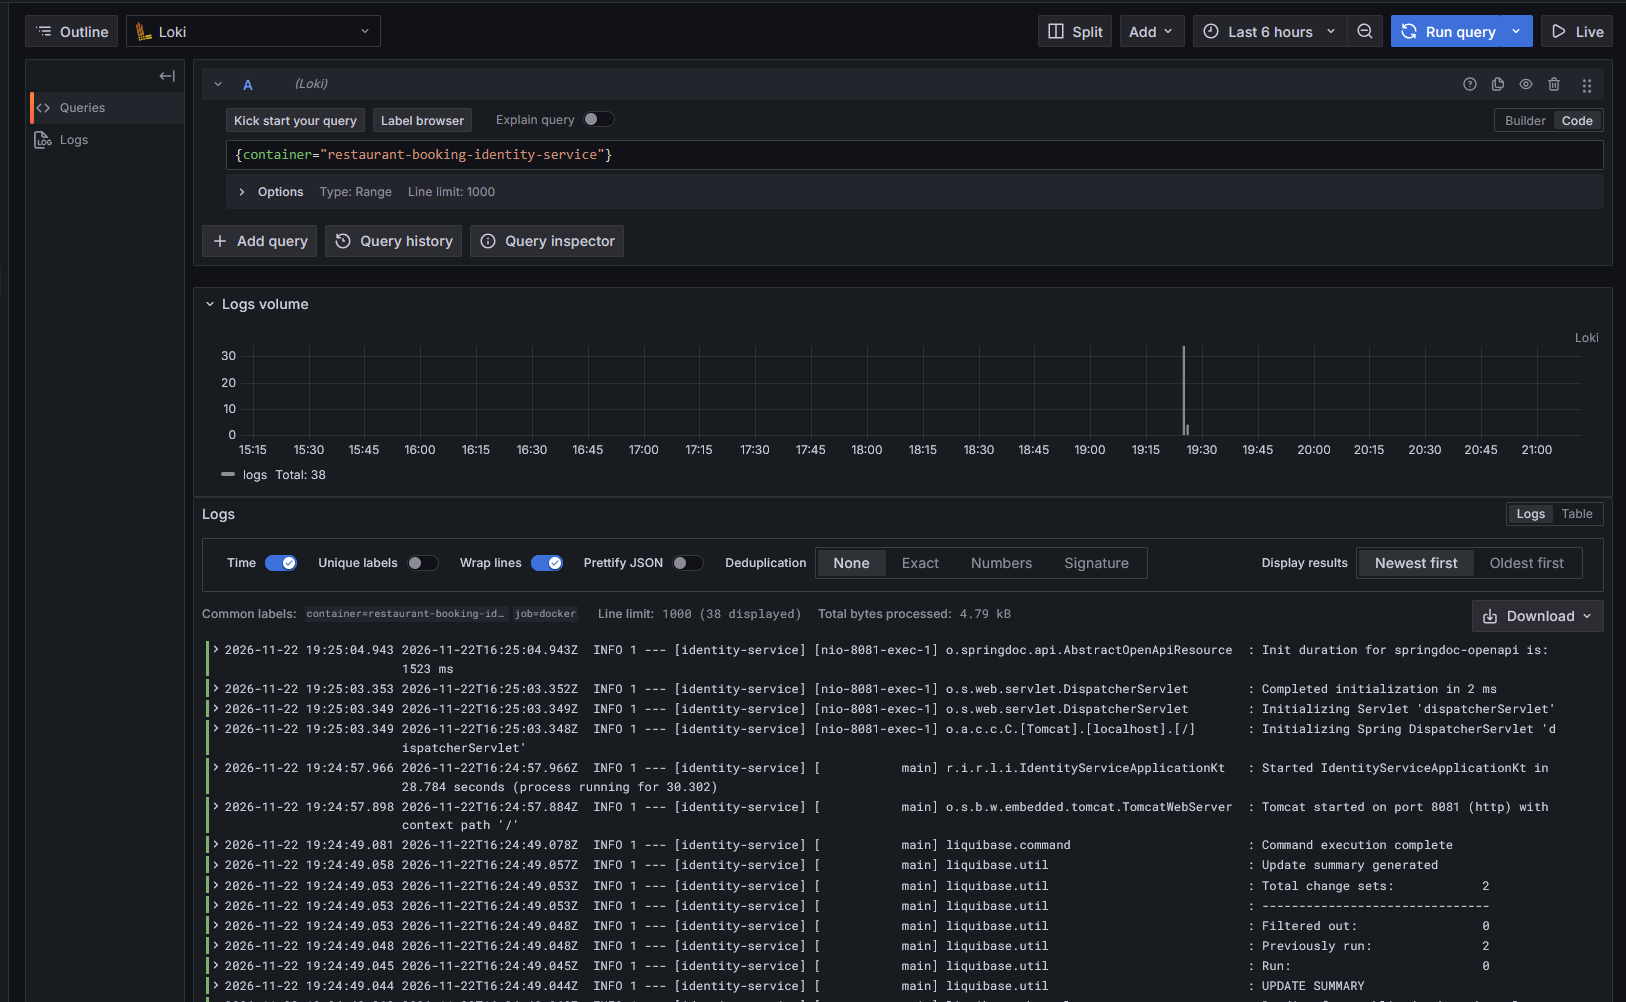
\includegraphics[width=\textwidth]{screenshots/identity-logs.png}\caption{Журналы identity-service в Grafana Explore}\end{figure}
\section{Вывод}
Развёрнута система мониторинга на базе Prometheus, Grafana, Loki и Alloy. Подготовленный дашборд отображает ресурсы виртуальной машины, доступность четырёх микросервисов и журналы контейнеров. Подключение обоих источников данных и работоспособность дашборда проверены на виртуальной машине.
\end{document}
